% Created by tikzDevice version 0.12
% !TEX encoding = UTF-8 Unicode
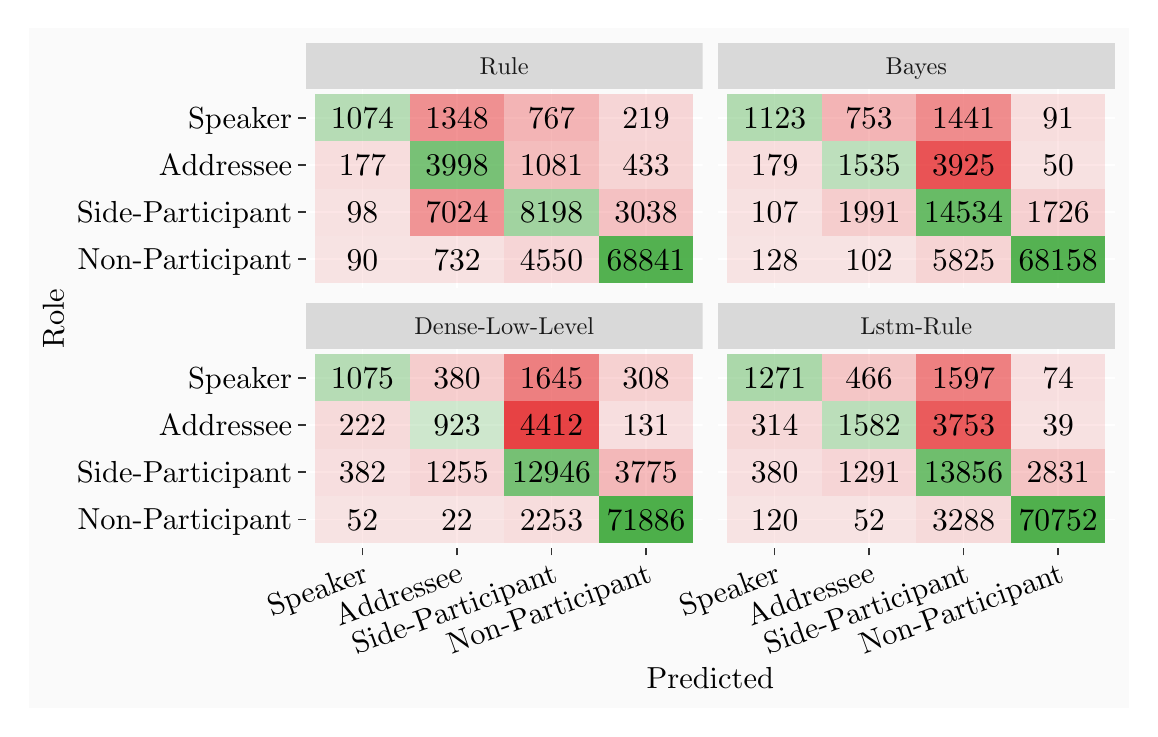
\begin{tikzpicture}[x=1pt,y=1pt]
\definecolor{fillColor}{RGB}{255,255,255}
\path[use as bounding box,fill=fillColor,fill opacity=0.00] (0,0) rectangle (398.34,246.17);
\begin{scope}
\path[clip] (  0.00,  0.00) rectangle (398.34,246.17);
\definecolor{drawColor}{RGB}{255,255,255}
\definecolor{fillColor}{gray}{0.98}

\path[draw=drawColor,line width= 0.6pt,line join=round,line cap=round,fill=fillColor] (  0.00,  0.00) rectangle (398.34,246.17);
\end{scope}
\begin{scope}
\path[clip] (100.50,152.22) rectangle (243.92,223.87);
\definecolor{drawColor}{RGB}{255,255,255}

\path[draw=drawColor,line width= 0.6pt,line join=round] (100.50,162.46) --
	(243.92,162.46);

\path[draw=drawColor,line width= 0.6pt,line join=round] (100.50,179.51) --
	(243.92,179.51);

\path[draw=drawColor,line width= 0.6pt,line join=round] (100.50,196.57) --
	(243.92,196.57);

\path[draw=drawColor,line width= 0.6pt,line join=round] (100.50,213.63) --
	(243.92,213.63);

\path[draw=drawColor,line width= 0.6pt,line join=round] (120.98,152.22) --
	(120.98,223.87);

\path[draw=drawColor,line width= 0.6pt,line join=round] (155.13,152.22) --
	(155.13,223.87);

\path[draw=drawColor,line width= 0.6pt,line join=round] (189.28,152.22) --
	(189.28,223.87);

\path[draw=drawColor,line width= 0.6pt,line join=round] (223.43,152.22) --
	(223.43,223.87);
\definecolor{fillColor}{RGB}{77,175,74}

\path[fill=fillColor,fill opacity=0.39] (103.91,205.10) rectangle (138.06,222.16);
\definecolor{fillColor}{RGB}{228,26,28}

\path[fill=fillColor,fill opacity=0.47] (138.06,205.10) rectangle (172.21,222.16);
\definecolor{fillColor}{RGB}{228,26,28}

\path[fill=fillColor,fill opacity=0.31] (172.21,205.10) rectangle (206.35,222.16);
\definecolor{fillColor}{RGB}{228,26,28}

\path[fill=fillColor,fill opacity=0.16] (206.35,205.10) rectangle (240.50,222.16);
\definecolor{fillColor}{RGB}{228,26,28}

\path[fill=fillColor,fill opacity=0.13] (103.91,188.04) rectangle (138.06,205.10);
\definecolor{fillColor}{RGB}{77,175,74}

\path[fill=fillColor,fill opacity=0.75] (138.06,188.04) rectangle (172.21,205.10);
\definecolor{fillColor}{RGB}{228,26,28}

\path[fill=fillColor,fill opacity=0.27] (172.21,188.04) rectangle (206.35,205.10);
\definecolor{fillColor}{RGB}{228,26,28}

\path[fill=fillColor,fill opacity=0.17] (206.35,188.04) rectangle (240.50,205.10);
\definecolor{fillColor}{RGB}{228,26,28}

\path[fill=fillColor,fill opacity=0.11] (103.91,170.99) rectangle (138.06,188.04);
\definecolor{fillColor}{RGB}{228,26,28}

\path[fill=fillColor,fill opacity=0.45] (138.06,170.99) rectangle (172.21,188.04);
\definecolor{fillColor}{RGB}{77,175,74}

\path[fill=fillColor,fill opacity=0.51] (172.21,170.99) rectangle (206.35,188.04);
\definecolor{fillColor}{RGB}{228,26,28}

\path[fill=fillColor,fill opacity=0.25] (206.35,170.99) rectangle (240.50,188.04);
\definecolor{fillColor}{RGB}{228,26,28}

\path[fill=fillColor,fill opacity=0.10] (103.91,153.93) rectangle (138.06,170.99);
\definecolor{fillColor}{RGB}{228,26,28}

\path[fill=fillColor,fill opacity=0.11] (138.06,153.93) rectangle (172.21,170.99);
\definecolor{fillColor}{RGB}{228,26,28}

\path[fill=fillColor,fill opacity=0.16] (172.21,153.93) rectangle (206.35,170.99);
\definecolor{fillColor}{RGB}{77,175,74}

\path[fill=fillColor,fill opacity=0.96] (206.35,153.93) rectangle (240.50,170.99);
\definecolor{drawColor}{RGB}{0,0,0}

\node[text=drawColor,anchor=base,inner sep=0pt, outer sep=0pt, scale=  1.14] at (120.98,209.71) {1074};

\node[text=drawColor,anchor=base,inner sep=0pt, outer sep=0pt, scale=  1.14] at (155.13,209.71) {1348};

\node[text=drawColor,anchor=base,inner sep=0pt, outer sep=0pt, scale=  1.14] at (189.28,209.71) {767};

\node[text=drawColor,anchor=base,inner sep=0pt, outer sep=0pt, scale=  1.14] at (223.43,209.71) {219};

\node[text=drawColor,anchor=base,inner sep=0pt, outer sep=0pt, scale=  1.14] at (120.98,192.66) {177};

\node[text=drawColor,anchor=base,inner sep=0pt, outer sep=0pt, scale=  1.14] at (155.13,192.66) {3998};

\node[text=drawColor,anchor=base,inner sep=0pt, outer sep=0pt, scale=  1.14] at (189.28,192.66) {1081};

\node[text=drawColor,anchor=base,inner sep=0pt, outer sep=0pt, scale=  1.14] at (223.43,192.66) {433};

\node[text=drawColor,anchor=base,inner sep=0pt, outer sep=0pt, scale=  1.14] at (120.98,175.60) {98};

\node[text=drawColor,anchor=base,inner sep=0pt, outer sep=0pt, scale=  1.14] at (155.13,175.60) {7024};

\node[text=drawColor,anchor=base,inner sep=0pt, outer sep=0pt, scale=  1.14] at (189.28,175.60) {8198};

\node[text=drawColor,anchor=base,inner sep=0pt, outer sep=0pt, scale=  1.14] at (223.43,175.60) {3038};

\node[text=drawColor,anchor=base,inner sep=0pt, outer sep=0pt, scale=  1.14] at (120.98,158.54) {90};

\node[text=drawColor,anchor=base,inner sep=0pt, outer sep=0pt, scale=  1.14] at (155.13,158.54) {732};

\node[text=drawColor,anchor=base,inner sep=0pt, outer sep=0pt, scale=  1.14] at (189.28,158.54) {4550};

\node[text=drawColor,anchor=base,inner sep=0pt, outer sep=0pt, scale=  1.14] at (223.43,158.54) {68841};
\end{scope}
\begin{scope}
\path[clip] (100.50, 58.27) rectangle (243.92,129.92);
\definecolor{drawColor}{RGB}{255,255,255}

\path[draw=drawColor,line width= 0.6pt,line join=round] (100.50, 68.50) --
	(243.92, 68.50);

\path[draw=drawColor,line width= 0.6pt,line join=round] (100.50, 85.56) --
	(243.92, 85.56);

\path[draw=drawColor,line width= 0.6pt,line join=round] (100.50,102.62) --
	(243.92,102.62);

\path[draw=drawColor,line width= 0.6pt,line join=round] (100.50,119.68) --
	(243.92,119.68);

\path[draw=drawColor,line width= 0.6pt,line join=round] (120.98, 58.27) --
	(120.98,129.92);

\path[draw=drawColor,line width= 0.6pt,line join=round] (155.13, 58.27) --
	(155.13,129.92);

\path[draw=drawColor,line width= 0.6pt,line join=round] (189.28, 58.27) --
	(189.28,129.92);

\path[draw=drawColor,line width= 0.6pt,line join=round] (223.43, 58.27) --
	(223.43,129.92);
\definecolor{fillColor}{RGB}{77,175,74}

\path[fill=fillColor,fill opacity=0.39] (103.91,111.15) rectangle (138.06,128.21);
\definecolor{fillColor}{RGB}{228,26,28}

\path[fill=fillColor,fill opacity=0.20] (138.06,111.15) rectangle (172.21,128.21);
\definecolor{fillColor}{RGB}{228,26,28}

\path[fill=fillColor,fill opacity=0.55] (172.21,111.15) rectangle (206.35,128.21);
\definecolor{fillColor}{RGB}{228,26,28}

\path[fill=fillColor,fill opacity=0.18] (206.35,111.15) rectangle (240.50,128.21);
\definecolor{fillColor}{RGB}{228,26,28}

\path[fill=fillColor,fill opacity=0.14] (103.91, 94.09) rectangle (138.06,111.15);
\definecolor{fillColor}{RGB}{77,175,74}

\path[fill=fillColor,fill opacity=0.25] (138.06, 94.09) rectangle (172.21,111.15);
\definecolor{fillColor}{RGB}{228,26,28}

\path[fill=fillColor,fill opacity=0.82] (172.21, 94.09) rectangle (206.35,111.15);
\definecolor{fillColor}{RGB}{228,26,28}

\path[fill=fillColor,fill opacity=0.12] (206.35, 94.09) rectangle (240.50,111.15);
\definecolor{fillColor}{RGB}{228,26,28}

\path[fill=fillColor,fill opacity=0.12] (103.91, 77.03) rectangle (138.06, 94.09);
\definecolor{fillColor}{RGB}{228,26,28}

\path[fill=fillColor,fill opacity=0.16] (138.06, 77.03) rectangle (172.21, 94.09);
\definecolor{fillColor}{RGB}{77,175,74}

\path[fill=fillColor,fill opacity=0.76] (172.21, 77.03) rectangle (206.35, 94.09);
\definecolor{fillColor}{RGB}{228,26,28}

\path[fill=fillColor,fill opacity=0.29] (206.35, 77.03) rectangle (240.50, 94.09);
\definecolor{fillColor}{RGB}{228,26,28}

\path[fill=fillColor,fill opacity=0.10] (103.91, 59.97) rectangle (138.06, 77.03);

\path[fill=fillColor,fill opacity=0.10] (138.06, 59.97) rectangle (172.21, 77.03);
\definecolor{fillColor}{RGB}{228,26,28}

\path[fill=fillColor,fill opacity=0.13] (172.21, 59.97) rectangle (206.35, 77.03);
\definecolor{fillColor}{RGB}{77,175,74}

\path[fill=fillColor] (206.35, 59.97) rectangle (240.50, 77.03);
\definecolor{drawColor}{RGB}{0,0,0}

\node[text=drawColor,anchor=base,inner sep=0pt, outer sep=0pt, scale=  1.14] at (120.98,115.76) {1075};

\node[text=drawColor,anchor=base,inner sep=0pt, outer sep=0pt, scale=  1.14] at (155.13,115.76) {380};

\node[text=drawColor,anchor=base,inner sep=0pt, outer sep=0pt, scale=  1.14] at (189.28,115.76) {1645};

\node[text=drawColor,anchor=base,inner sep=0pt, outer sep=0pt, scale=  1.14] at (223.43,115.76) {308};

\node[text=drawColor,anchor=base,inner sep=0pt, outer sep=0pt, scale=  1.14] at (120.98, 98.70) {222};

\node[text=drawColor,anchor=base,inner sep=0pt, outer sep=0pt, scale=  1.14] at (155.13, 98.70) {923};

\node[text=drawColor,anchor=base,inner sep=0pt, outer sep=0pt, scale=  1.14] at (189.28, 98.70) {4412};

\node[text=drawColor,anchor=base,inner sep=0pt, outer sep=0pt, scale=  1.14] at (223.43, 98.70) {131};

\node[text=drawColor,anchor=base,inner sep=0pt, outer sep=0pt, scale=  1.14] at (120.98, 81.64) {382};

\node[text=drawColor,anchor=base,inner sep=0pt, outer sep=0pt, scale=  1.14] at (155.13, 81.64) {1255};

\node[text=drawColor,anchor=base,inner sep=0pt, outer sep=0pt, scale=  1.14] at (189.28, 81.64) {12946};

\node[text=drawColor,anchor=base,inner sep=0pt, outer sep=0pt, scale=  1.14] at (223.43, 81.64) {3775};

\node[text=drawColor,anchor=base,inner sep=0pt, outer sep=0pt, scale=  1.14] at (120.98, 64.58) {52};

\node[text=drawColor,anchor=base,inner sep=0pt, outer sep=0pt, scale=  1.14] at (155.13, 64.58) {22};

\node[text=drawColor,anchor=base,inner sep=0pt, outer sep=0pt, scale=  1.14] at (189.28, 64.58) {2253};

\node[text=drawColor,anchor=base,inner sep=0pt, outer sep=0pt, scale=  1.14] at (223.43, 64.58) {71886};
\end{scope}
\begin{scope}
\path[clip] (249.42,152.22) rectangle (392.84,223.87);
\definecolor{drawColor}{RGB}{255,255,255}

\path[draw=drawColor,line width= 0.6pt,line join=round] (249.42,162.46) --
	(392.84,162.46);

\path[draw=drawColor,line width= 0.6pt,line join=round] (249.42,179.51) --
	(392.84,179.51);

\path[draw=drawColor,line width= 0.6pt,line join=round] (249.42,196.57) --
	(392.84,196.57);

\path[draw=drawColor,line width= 0.6pt,line join=round] (249.42,213.63) --
	(392.84,213.63);

\path[draw=drawColor,line width= 0.6pt,line join=round] (269.91,152.22) --
	(269.91,223.87);

\path[draw=drawColor,line width= 0.6pt,line join=round] (304.05,152.22) --
	(304.05,223.87);

\path[draw=drawColor,line width= 0.6pt,line join=round] (338.20,152.22) --
	(338.20,223.87);

\path[draw=drawColor,line width= 0.6pt,line join=round] (372.35,152.22) --
	(372.35,223.87);
\definecolor{fillColor}{RGB}{77,175,74}

\path[fill=fillColor,fill opacity=0.41] (252.83,205.10) rectangle (286.98,222.16);
\definecolor{fillColor}{RGB}{228,26,28}

\path[fill=fillColor,fill opacity=0.31] (286.98,205.10) rectangle (321.13,222.16);
\definecolor{fillColor}{RGB}{228,26,28}

\path[fill=fillColor,fill opacity=0.49] (321.13,205.10) rectangle (355.28,222.16);
\definecolor{fillColor}{RGB}{228,26,28}

\path[fill=fillColor,fill opacity=0.13] (355.28,205.10) rectangle (389.42,222.16);
\definecolor{fillColor}{RGB}{228,26,28}

\path[fill=fillColor,fill opacity=0.13] (252.83,188.04) rectangle (286.98,205.10);
\definecolor{fillColor}{RGB}{77,175,74}

\path[fill=fillColor,fill opacity=0.35] (286.98,188.04) rectangle (321.13,205.10);
\definecolor{fillColor}{RGB}{228,26,28}

\path[fill=fillColor,fill opacity=0.74] (321.13,188.04) rectangle (355.28,205.10);
\definecolor{fillColor}{RGB}{228,26,28}

\path[fill=fillColor,fill opacity=0.11] (355.28,188.04) rectangle (389.42,205.10);
\definecolor{fillColor}{RGB}{228,26,28}

\path[fill=fillColor,fill opacity=0.11] (252.83,170.99) rectangle (286.98,188.04);
\definecolor{fillColor}{RGB}{228,26,28}

\path[fill=fillColor,fill opacity=0.20] (286.98,170.99) rectangle (321.13,188.04);
\definecolor{fillColor}{RGB}{77,175,74}

\path[fill=fillColor,fill opacity=0.84] (321.13,170.99) rectangle (355.28,188.04);
\definecolor{fillColor}{RGB}{228,26,28}

\path[fill=fillColor,fill opacity=0.19] (355.28,170.99) rectangle (389.42,188.04);
\definecolor{fillColor}{RGB}{228,26,28}

\path[fill=fillColor,fill opacity=0.10] (252.83,153.93) rectangle (286.98,170.99);

\path[fill=fillColor,fill opacity=0.10] (286.98,153.93) rectangle (321.13,170.99);
\definecolor{fillColor}{RGB}{228,26,28}

\path[fill=fillColor,fill opacity=0.17] (321.13,153.93) rectangle (355.28,170.99);
\definecolor{fillColor}{RGB}{77,175,74}

\path[fill=fillColor,fill opacity=0.95] (355.28,153.93) rectangle (389.42,170.99);
\definecolor{drawColor}{RGB}{0,0,0}

\node[text=drawColor,anchor=base,inner sep=0pt, outer sep=0pt, scale=  1.14] at (269.91,209.71) {1123};

\node[text=drawColor,anchor=base,inner sep=0pt, outer sep=0pt, scale=  1.14] at (304.05,209.71) {753};

\node[text=drawColor,anchor=base,inner sep=0pt, outer sep=0pt, scale=  1.14] at (338.20,209.71) {1441};

\node[text=drawColor,anchor=base,inner sep=0pt, outer sep=0pt, scale=  1.14] at (372.35,209.71) {91};

\node[text=drawColor,anchor=base,inner sep=0pt, outer sep=0pt, scale=  1.14] at (269.91,192.66) {179};

\node[text=drawColor,anchor=base,inner sep=0pt, outer sep=0pt, scale=  1.14] at (304.05,192.66) {1535};

\node[text=drawColor,anchor=base,inner sep=0pt, outer sep=0pt, scale=  1.14] at (338.20,192.66) {3925};

\node[text=drawColor,anchor=base,inner sep=0pt, outer sep=0pt, scale=  1.14] at (372.35,192.66) {50};

\node[text=drawColor,anchor=base,inner sep=0pt, outer sep=0pt, scale=  1.14] at (269.91,175.60) {107};

\node[text=drawColor,anchor=base,inner sep=0pt, outer sep=0pt, scale=  1.14] at (304.05,175.60) {1991};

\node[text=drawColor,anchor=base,inner sep=0pt, outer sep=0pt, scale=  1.14] at (338.20,175.60) {14534};

\node[text=drawColor,anchor=base,inner sep=0pt, outer sep=0pt, scale=  1.14] at (372.35,175.60) {1726};

\node[text=drawColor,anchor=base,inner sep=0pt, outer sep=0pt, scale=  1.14] at (269.91,158.54) {128};

\node[text=drawColor,anchor=base,inner sep=0pt, outer sep=0pt, scale=  1.14] at (304.05,158.54) {102};

\node[text=drawColor,anchor=base,inner sep=0pt, outer sep=0pt, scale=  1.14] at (338.20,158.54) {5825};

\node[text=drawColor,anchor=base,inner sep=0pt, outer sep=0pt, scale=  1.14] at (372.35,158.54) {68158};
\end{scope}
\begin{scope}
\path[clip] (249.42, 58.27) rectangle (392.84,129.92);
\definecolor{drawColor}{RGB}{255,255,255}

\path[draw=drawColor,line width= 0.6pt,line join=round] (249.42, 68.50) --
	(392.84, 68.50);

\path[draw=drawColor,line width= 0.6pt,line join=round] (249.42, 85.56) --
	(392.84, 85.56);

\path[draw=drawColor,line width= 0.6pt,line join=round] (249.42,102.62) --
	(392.84,102.62);

\path[draw=drawColor,line width= 0.6pt,line join=round] (249.42,119.68) --
	(392.84,119.68);

\path[draw=drawColor,line width= 0.6pt,line join=round] (269.91, 58.27) --
	(269.91,129.92);

\path[draw=drawColor,line width= 0.6pt,line join=round] (304.05, 58.27) --
	(304.05,129.92);

\path[draw=drawColor,line width= 0.6pt,line join=round] (338.20, 58.27) --
	(338.20,129.92);

\path[draw=drawColor,line width= 0.6pt,line join=round] (372.35, 58.27) --
	(372.35,129.92);
\definecolor{fillColor}{RGB}{77,175,74}

\path[fill=fillColor,fill opacity=0.45] (252.83,111.15) rectangle (286.98,128.21);
\definecolor{fillColor}{RGB}{228,26,28}

\path[fill=fillColor,fill opacity=0.23] (286.98,111.15) rectangle (321.13,128.21);
\definecolor{fillColor}{RGB}{228,26,28}

\path[fill=fillColor,fill opacity=0.54] (321.13,111.15) rectangle (355.28,128.21);
\definecolor{fillColor}{RGB}{228,26,28}

\path[fill=fillColor,fill opacity=0.12] (355.28,111.15) rectangle (389.42,128.21);
\definecolor{fillColor}{RGB}{228,26,28}

\path[fill=fillColor,fill opacity=0.15] (252.83, 94.09) rectangle (286.98,111.15);
\definecolor{fillColor}{RGB}{77,175,74}

\path[fill=fillColor,fill opacity=0.36] (286.98, 94.09) rectangle (321.13,111.15);
\definecolor{fillColor}{RGB}{228,26,28}

\path[fill=fillColor,fill opacity=0.71] (321.13, 94.09) rectangle (355.28,111.15);
\definecolor{fillColor}{RGB}{228,26,28}

\path[fill=fillColor,fill opacity=0.11] (355.28, 94.09) rectangle (389.42,111.15);
\definecolor{fillColor}{RGB}{228,26,28}

\path[fill=fillColor,fill opacity=0.12] (252.83, 77.03) rectangle (286.98, 94.09);
\definecolor{fillColor}{RGB}{228,26,28}

\path[fill=fillColor,fill opacity=0.16] (286.98, 77.03) rectangle (321.13, 94.09);
\definecolor{fillColor}{RGB}{77,175,74}

\path[fill=fillColor,fill opacity=0.80] (321.13, 77.03) rectangle (355.28, 94.09);
\definecolor{fillColor}{RGB}{228,26,28}

\path[fill=fillColor,fill opacity=0.24] (355.28, 77.03) rectangle (389.42, 94.09);
\definecolor{fillColor}{RGB}{228,26,28}

\path[fill=fillColor,fill opacity=0.10] (252.83, 59.97) rectangle (286.98, 77.03);

\path[fill=fillColor,fill opacity=0.10] (286.98, 59.97) rectangle (321.13, 77.03);
\definecolor{fillColor}{RGB}{228,26,28}

\path[fill=fillColor,fill opacity=0.14] (321.13, 59.97) rectangle (355.28, 77.03);
\definecolor{fillColor}{RGB}{77,175,74}

\path[fill=fillColor,fill opacity=0.98] (355.28, 59.97) rectangle (389.42, 77.03);
\definecolor{drawColor}{RGB}{0,0,0}

\node[text=drawColor,anchor=base,inner sep=0pt, outer sep=0pt, scale=  1.14] at (269.91,115.76) {1271};

\node[text=drawColor,anchor=base,inner sep=0pt, outer sep=0pt, scale=  1.14] at (304.05,115.76) {466};

\node[text=drawColor,anchor=base,inner sep=0pt, outer sep=0pt, scale=  1.14] at (338.20,115.76) {1597};

\node[text=drawColor,anchor=base,inner sep=0pt, outer sep=0pt, scale=  1.14] at (372.35,115.76) {74};

\node[text=drawColor,anchor=base,inner sep=0pt, outer sep=0pt, scale=  1.14] at (269.91, 98.70) {314};

\node[text=drawColor,anchor=base,inner sep=0pt, outer sep=0pt, scale=  1.14] at (304.05, 98.70) {1582};

\node[text=drawColor,anchor=base,inner sep=0pt, outer sep=0pt, scale=  1.14] at (338.20, 98.70) {3753};

\node[text=drawColor,anchor=base,inner sep=0pt, outer sep=0pt, scale=  1.14] at (372.35, 98.70) {39};

\node[text=drawColor,anchor=base,inner sep=0pt, outer sep=0pt, scale=  1.14] at (269.91, 81.64) {380};

\node[text=drawColor,anchor=base,inner sep=0pt, outer sep=0pt, scale=  1.14] at (304.05, 81.64) {1291};

\node[text=drawColor,anchor=base,inner sep=0pt, outer sep=0pt, scale=  1.14] at (338.20, 81.64) {13856};

\node[text=drawColor,anchor=base,inner sep=0pt, outer sep=0pt, scale=  1.14] at (372.35, 81.64) {2831};

\node[text=drawColor,anchor=base,inner sep=0pt, outer sep=0pt, scale=  1.14] at (269.91, 64.58) {120};

\node[text=drawColor,anchor=base,inner sep=0pt, outer sep=0pt, scale=  1.14] at (304.05, 64.58) {52};

\node[text=drawColor,anchor=base,inner sep=0pt, outer sep=0pt, scale=  1.14] at (338.20, 64.58) {3288};

\node[text=drawColor,anchor=base,inner sep=0pt, outer sep=0pt, scale=  1.14] at (372.35, 64.58) {70752};
\end{scope}
\begin{scope}
\path[clip] (100.50,129.92) rectangle (243.92,146.72);
\definecolor{fillColor}{gray}{0.85}

\path[fill=fillColor] (100.50,129.92) rectangle (243.92,146.72);
\definecolor{drawColor}{gray}{0.10}

\node[text=drawColor,anchor=base,inner sep=0pt, outer sep=0pt, scale=  0.88] at (172.21,135.29) {Dense-Low-Level};
\end{scope}
\begin{scope}
\path[clip] (249.42,129.92) rectangle (392.84,146.72);
\definecolor{fillColor}{gray}{0.85}

\path[fill=fillColor] (249.42,129.92) rectangle (392.84,146.72);
\definecolor{drawColor}{gray}{0.10}

\node[text=drawColor,anchor=base,inner sep=0pt, outer sep=0pt, scale=  0.88] at (321.13,135.29) {Lstm-Rule};
\end{scope}
\begin{scope}
\path[clip] (100.50,223.87) rectangle (243.92,240.67);
\definecolor{fillColor}{gray}{0.85}

\path[fill=fillColor] (100.50,223.87) rectangle (243.92,240.67);
\definecolor{drawColor}{gray}{0.10}

\node[text=drawColor,anchor=base,inner sep=0pt, outer sep=0pt, scale=  0.88] at (172.21,229.24) {Rule};
\end{scope}
\begin{scope}
\path[clip] (249.42,223.87) rectangle (392.84,240.67);
\definecolor{fillColor}{gray}{0.85}

\path[fill=fillColor] (249.42,223.87) rectangle (392.84,240.67);
\definecolor{drawColor}{gray}{0.10}

\node[text=drawColor,anchor=base,inner sep=0pt, outer sep=0pt, scale=  0.88] at (321.13,229.24) {Bayes};
\end{scope}
\begin{scope}
\path[clip] (  0.00,  0.00) rectangle (398.34,246.17);
\definecolor{drawColor}{gray}{0.20}

\path[draw=drawColor,line width= 0.6pt,line join=round] (120.98, 55.52) --
	(120.98, 58.27);

\path[draw=drawColor,line width= 0.6pt,line join=round] (155.13, 55.52) --
	(155.13, 58.27);

\path[draw=drawColor,line width= 0.6pt,line join=round] (189.28, 55.52) --
	(189.28, 58.27);

\path[draw=drawColor,line width= 0.6pt,line join=round] (223.43, 55.52) --
	(223.43, 58.27);
\end{scope}
\begin{scope}
\path[clip] (  0.00,  0.00) rectangle (398.34,246.17);
\definecolor{drawColor}{RGB}{0,0,0}

\node[text=drawColor,rotate= 20.00,anchor=base east,inner sep=0pt, outer sep=0pt, scale=  1.10] at (123.58, 46.20) {Speaker};

\node[text=drawColor,rotate= 20.00,anchor=base east,inner sep=0pt, outer sep=0pt, scale=  1.10] at (157.72, 46.20) {Addressee};

\node[text=drawColor,rotate= 20.00,anchor=base east,inner sep=0pt, outer sep=0pt, scale=  1.10] at (191.87, 46.20) {Side-Participant};

\node[text=drawColor,rotate= 20.00,anchor=base east,inner sep=0pt, outer sep=0pt, scale=  1.10] at (226.02, 46.20) {Non-Participant};
\end{scope}
\begin{scope}
\path[clip] (  0.00,  0.00) rectangle (398.34,246.17);
\definecolor{drawColor}{gray}{0.20}

\path[draw=drawColor,line width= 0.6pt,line join=round] (269.91, 55.52) --
	(269.91, 58.27);

\path[draw=drawColor,line width= 0.6pt,line join=round] (304.05, 55.52) --
	(304.05, 58.27);

\path[draw=drawColor,line width= 0.6pt,line join=round] (338.20, 55.52) --
	(338.20, 58.27);

\path[draw=drawColor,line width= 0.6pt,line join=round] (372.35, 55.52) --
	(372.35, 58.27);
\end{scope}
\begin{scope}
\path[clip] (  0.00,  0.00) rectangle (398.34,246.17);
\definecolor{drawColor}{RGB}{0,0,0}

\node[text=drawColor,rotate= 20.00,anchor=base east,inner sep=0pt, outer sep=0pt, scale=  1.10] at (272.50, 46.20) {Speaker};

\node[text=drawColor,rotate= 20.00,anchor=base east,inner sep=0pt, outer sep=0pt, scale=  1.10] at (306.65, 46.20) {Addressee};

\node[text=drawColor,rotate= 20.00,anchor=base east,inner sep=0pt, outer sep=0pt, scale=  1.10] at (340.79, 46.20) {Side-Participant};

\node[text=drawColor,rotate= 20.00,anchor=base east,inner sep=0pt, outer sep=0pt, scale=  1.10] at (374.94, 46.20) {Non-Participant};
\end{scope}
\begin{scope}
\path[clip] (  0.00,  0.00) rectangle (398.34,246.17);
\definecolor{drawColor}{RGB}{0,0,0}

\node[text=drawColor,anchor=base east,inner sep=0pt, outer sep=0pt, scale=  1.10] at ( 95.55,158.67) {Non-Participant};

\node[text=drawColor,anchor=base east,inner sep=0pt, outer sep=0pt, scale=  1.10] at ( 95.55,175.73) {Side-Participant};

\node[text=drawColor,anchor=base east,inner sep=0pt, outer sep=0pt, scale=  1.10] at ( 95.55,192.79) {Addressee};

\node[text=drawColor,anchor=base east,inner sep=0pt, outer sep=0pt, scale=  1.10] at ( 95.55,209.85) {Speaker};
\end{scope}
\begin{scope}
\path[clip] (  0.00,  0.00) rectangle (398.34,246.17);
\definecolor{drawColor}{gray}{0.20}

\path[draw=drawColor,line width= 0.6pt,line join=round] ( 97.75,162.46) --
	(100.50,162.46);

\path[draw=drawColor,line width= 0.6pt,line join=round] ( 97.75,179.51) --
	(100.50,179.51);

\path[draw=drawColor,line width= 0.6pt,line join=round] ( 97.75,196.57) --
	(100.50,196.57);

\path[draw=drawColor,line width= 0.6pt,line join=round] ( 97.75,213.63) --
	(100.50,213.63);
\end{scope}
\begin{scope}
\path[clip] (  0.00,  0.00) rectangle (398.34,246.17);
\definecolor{drawColor}{RGB}{0,0,0}

\node[text=drawColor,anchor=base east,inner sep=0pt, outer sep=0pt, scale=  1.10] at ( 95.55, 64.71) {Non-Participant};

\node[text=drawColor,anchor=base east,inner sep=0pt, outer sep=0pt, scale=  1.10] at ( 95.55, 81.77) {Side-Participant};

\node[text=drawColor,anchor=base east,inner sep=0pt, outer sep=0pt, scale=  1.10] at ( 95.55, 98.83) {Addressee};

\node[text=drawColor,anchor=base east,inner sep=0pt, outer sep=0pt, scale=  1.10] at ( 95.55,115.89) {Speaker};
\end{scope}
\begin{scope}
\path[clip] (  0.00,  0.00) rectangle (398.34,246.17);
\definecolor{drawColor}{gray}{0.20}

\path[draw=drawColor,line width= 0.6pt,line join=round] ( 97.75, 68.50) --
	(100.50, 68.50);

\path[draw=drawColor,line width= 0.6pt,line join=round] ( 97.75, 85.56) --
	(100.50, 85.56);

\path[draw=drawColor,line width= 0.6pt,line join=round] ( 97.75,102.62) --
	(100.50,102.62);

\path[draw=drawColor,line width= 0.6pt,line join=round] ( 97.75,119.68) --
	(100.50,119.68);
\end{scope}
\begin{scope}
\path[clip] (  0.00,  0.00) rectangle (398.34,246.17);
\definecolor{drawColor}{RGB}{0,0,0}

\node[text=drawColor,anchor=base,inner sep=0pt, outer sep=0pt, scale=  1.10] at (246.67,  7.44) {Predicted};
\end{scope}
\begin{scope}
\path[clip] (  0.00,  0.00) rectangle (398.34,246.17);
\definecolor{drawColor}{RGB}{0,0,0}

\node[text=drawColor,rotate= 90.00,anchor=base,inner sep=0pt, outer sep=0pt, scale=  1.10] at ( 13.08,141.07) {Role};
\end{scope}
\end{tikzpicture}
